% Options for packages loaded elsewhere
\PassOptionsToPackage{unicode}{hyperref}
\PassOptionsToPackage{hyphens}{url}
%
\documentclass[
  10pt,
  ignorenonframetext,
]{beamer}
\usepackage{pgfpages}
\setbeamertemplate{caption}[numbered]
\setbeamertemplate{caption label separator}{: }
\setbeamercolor{caption name}{fg=normal text.fg}
\beamertemplatenavigationsymbolsempty
% Prevent slide breaks in the middle of a paragraph
\widowpenalties 1 10000
\raggedbottom
\setbeamertemplate{part page}{
  \centering
  \begin{beamercolorbox}[sep=16pt,center]{part title}
    \usebeamerfont{part title}\insertpart\par
  \end{beamercolorbox}
}
\setbeamertemplate{section page}{
  \centering
  \begin{beamercolorbox}[sep=12pt,center]{part title}
    \usebeamerfont{section title}\insertsection\par
  \end{beamercolorbox}
}
\setbeamertemplate{subsection page}{
  \centering
  \begin{beamercolorbox}[sep=8pt,center]{part title}
    \usebeamerfont{subsection title}\insertsubsection\par
  \end{beamercolorbox}
}
\AtBeginPart{
  \frame{\partpage}
}
\AtBeginSection{
  \ifbibliography
  \else
    \frame{\sectionpage}
  \fi
}
\AtBeginSubsection{
  \frame{\subsectionpage}
}
\usepackage{amsmath,amssymb}
\usepackage{lmodern}
\usepackage{setspace}
\usepackage{iftex}
\ifPDFTeX
  \usepackage[T1]{fontenc}
  \usepackage[utf8]{inputenc}
  \usepackage{textcomp} % provide euro and other symbols
\else % if luatex or xetex
  \usepackage{unicode-math}
  \defaultfontfeatures{Scale=MatchLowercase}
  \defaultfontfeatures[\rmfamily]{Ligatures=TeX,Scale=1}
\fi
% Use upquote if available, for straight quotes in verbatim environments
\IfFileExists{upquote.sty}{\usepackage{upquote}}{}
\IfFileExists{microtype.sty}{% use microtype if available
  \usepackage[]{microtype}
  \UseMicrotypeSet[protrusion]{basicmath} % disable protrusion for tt fonts
}{}
\makeatletter
\@ifundefined{KOMAClassName}{% if non-KOMA class
  \IfFileExists{parskip.sty}{%
    \usepackage{parskip}
  }{% else
    \setlength{\parindent}{0pt}
    \setlength{\parskip}{6pt plus 2pt minus 1pt}}
}{% if KOMA class
  \KOMAoptions{parskip=half}}
\makeatother
\usepackage{xcolor}
\geometry{left = 1cm, right = 0.5cm, top = 0.5cm, bottom = 0.5cm}
\newif\ifbibliography
\usepackage{color}
\usepackage{fancyvrb}
\newcommand{\VerbBar}{|}
\newcommand{\VERB}{\Verb[commandchars=\\\{\}]}
\DefineVerbatimEnvironment{Highlighting}{Verbatim}{commandchars=\\\{\}}
% Add ',fontsize=\small' for more characters per line
\usepackage{framed}
\definecolor{shadecolor}{RGB}{248,248,248}
\newenvironment{Shaded}{\begin{snugshade}}{\end{snugshade}}
\newcommand{\AlertTok}[1]{\textcolor[rgb]{0.94,0.16,0.16}{#1}}
\newcommand{\AnnotationTok}[1]{\textcolor[rgb]{0.56,0.35,0.01}{\textbf{\textit{#1}}}}
\newcommand{\AttributeTok}[1]{\textcolor[rgb]{0.77,0.63,0.00}{#1}}
\newcommand{\BaseNTok}[1]{\textcolor[rgb]{0.00,0.00,0.81}{#1}}
\newcommand{\BuiltInTok}[1]{#1}
\newcommand{\CharTok}[1]{\textcolor[rgb]{0.31,0.60,0.02}{#1}}
\newcommand{\CommentTok}[1]{\textcolor[rgb]{0.56,0.35,0.01}{\textit{#1}}}
\newcommand{\CommentVarTok}[1]{\textcolor[rgb]{0.56,0.35,0.01}{\textbf{\textit{#1}}}}
\newcommand{\ConstantTok}[1]{\textcolor[rgb]{0.00,0.00,0.00}{#1}}
\newcommand{\ControlFlowTok}[1]{\textcolor[rgb]{0.13,0.29,0.53}{\textbf{#1}}}
\newcommand{\DataTypeTok}[1]{\textcolor[rgb]{0.13,0.29,0.53}{#1}}
\newcommand{\DecValTok}[1]{\textcolor[rgb]{0.00,0.00,0.81}{#1}}
\newcommand{\DocumentationTok}[1]{\textcolor[rgb]{0.56,0.35,0.01}{\textbf{\textit{#1}}}}
\newcommand{\ErrorTok}[1]{\textcolor[rgb]{0.64,0.00,0.00}{\textbf{#1}}}
\newcommand{\ExtensionTok}[1]{#1}
\newcommand{\FloatTok}[1]{\textcolor[rgb]{0.00,0.00,0.81}{#1}}
\newcommand{\FunctionTok}[1]{\textcolor[rgb]{0.00,0.00,0.00}{#1}}
\newcommand{\ImportTok}[1]{#1}
\newcommand{\InformationTok}[1]{\textcolor[rgb]{0.56,0.35,0.01}{\textbf{\textit{#1}}}}
\newcommand{\KeywordTok}[1]{\textcolor[rgb]{0.13,0.29,0.53}{\textbf{#1}}}
\newcommand{\NormalTok}[1]{#1}
\newcommand{\OperatorTok}[1]{\textcolor[rgb]{0.81,0.36,0.00}{\textbf{#1}}}
\newcommand{\OtherTok}[1]{\textcolor[rgb]{0.56,0.35,0.01}{#1}}
\newcommand{\PreprocessorTok}[1]{\textcolor[rgb]{0.56,0.35,0.01}{\textit{#1}}}
\newcommand{\RegionMarkerTok}[1]{#1}
\newcommand{\SpecialCharTok}[1]{\textcolor[rgb]{0.00,0.00,0.00}{#1}}
\newcommand{\SpecialStringTok}[1]{\textcolor[rgb]{0.31,0.60,0.02}{#1}}
\newcommand{\StringTok}[1]{\textcolor[rgb]{0.31,0.60,0.02}{#1}}
\newcommand{\VariableTok}[1]{\textcolor[rgb]{0.00,0.00,0.00}{#1}}
\newcommand{\VerbatimStringTok}[1]{\textcolor[rgb]{0.31,0.60,0.02}{#1}}
\newcommand{\WarningTok}[1]{\textcolor[rgb]{0.56,0.35,0.01}{\textbf{\textit{#1}}}}
\setlength{\emergencystretch}{3em} % prevent overfull lines
\providecommand{\tightlist}{%
  \setlength{\itemsep}{0pt}\setlength{\parskip}{0pt}}
\setcounter{secnumdepth}{-\maxdimen} % remove section numbering
\usepackage{float}
\usepackage{booktabs}
\usepackage{array}
\usepackage{longtable}
\usepackage{makecell}
\useinnertheme{rectangles}
\setbeamertemplate{itemize subitem}{\scriptsize$\diamond$}
\definecolor{blue}{RGB}{0,114,178}
\definecolor{red}{RGB}{213,94,0}
\definecolor{yellow}{RGB}{240,228,66}
\definecolor{green}{RGB}{0,158,115}
\ifLuaTeX
  \usepackage{selnolig}  % disable illegal ligatures
\fi
\IfFileExists{bookmark.sty}{\usepackage{bookmark}}{\usepackage{hyperref}}
\IfFileExists{xurl.sty}{\usepackage{xurl}}{} % add URL line breaks if available
\urlstyle{same} % disable monospaced font for URLs
\hypersetup{
  pdftitle={Introductory Statistics for Economics},
  pdfauthor={Duong Trinh},
  hidelinks,
  pdfcreator={LaTeX via pandoc}}

\title{Introductory Statistics for Economics}
\subtitle{ECON1013: LAB 3}
\author{Duong Trinh}
\date{Feb 2024}
\institute{University of Glasgow}

\begin{document}
\frame{\titlepage}

\setstretch{1.5}
\begin{frame}{Intro}
\protect\hypertarget{intro}{}
\begin{itemize}
\tightlist
\item
  Duong Trinh

  \begin{itemize}
  \tightlist
  \item
    PhD Student in Economics (Bayesian Microeconometrics)
  \item
    Email: \underline{Duong.Trinh@glasgow.ac.uk}
  \end{itemize}
\end{itemize}

\vspace{3mm}

\begin{itemize}
\tightlist
\item
  ECON1013-LB04

  \begin{itemize}
  \tightlist
  \item
    Monday 1-2 pm
  \item
    3 sessions (29-Jan, 12-Feb, 26-Feb)
  \end{itemize}
\item
  ECON1013-LB05

  \begin{itemize}
  \tightlist
  \item
    Tuesday 12-1 pm
  \item
    3 sessions (30-Jan, 13-Feb, 27-Feb)
  \end{itemize}
\item
  ECON1013-LB06

  \begin{itemize}
  \tightlist
  \item
    Tuesday 1-2 pm
  \item
    3 sessions (30-Jan, 13-Feb, 27-Feb)
  \end{itemize}
\end{itemize}

\vspace{3mm}
\end{frame}

\begin{frame}{Record Attendance}
\protect\hypertarget{record-attendance}{}
\end{frame}

\begin{frame}{Setup}
\protect\hypertarget{setup}{}
\begin{itemize}
\item
  Step 1: Download Lab materials from \textbf{Moodle} page
  \(\rightarrow\) Extract the folder in PC.
\item
  Step 2: Log in \textbf{Microsoft onedrive} using your student account
  \textcolor{blue}{https://onedrive.live.com/login/} and upload the
  folder above.
\item
  Step 3: Launch the \textbf{Excel} online
  \textcolor{blue}{https://www.office.com/launch/excel?auth=2}, which we
  will use for all lab sessions.
\end{itemize}
\end{frame}

\hypertarget{exercise-1.-confidence-intervals.}{%
\section{Exercise 1. Confidence
intervals.}\label{exercise-1.-confidence-intervals.}}

\begin{frame}{Exercise 1. Confidence intervals.}
\begin{itemize}
\tightlist
\item
  Data set: \texttt{testscores.xls}
\item
  About: A sample (\(n=200\)) of student test scores in Math and English

  \begin{itemize}
  \tightlist
  \item
    Minimal text score is 0 and maximal test score is 100.
  \end{itemize}
\end{itemize}
\end{frame}

\begin{frame}{Part 1. Confidence interval for the mean (\(\sigma\)
known).}
\protect\hypertarget{part-1.-confidence-interval-for-the-mean-sigma-known.}{}
We know that the population standard deviation \(\sigma_\mu\) for
variable ``English'' is equal to \(4.6\).

\begin{enumerate}
\item
  Find the sample mean for the variable ``English''.
\item
  Find the standard error of the sample mean for the variable
  ``English''.
\item
  Find the margin of error at the \(95\%\) confidence level.
\item
  Find the \(95\%\) confidence interval for the mean.
\end{enumerate}

Hint: \(SE=0.33\), \(ME=0.64\).
\end{frame}

\begin{frame}{Where we currently are}
\protect\hypertarget{where-we-currently-are}{}
\begin{center}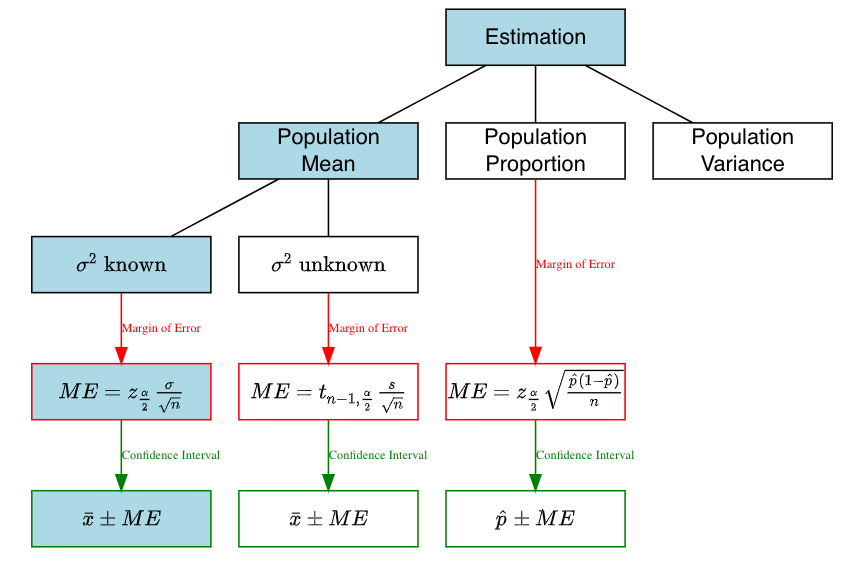
\includegraphics[width=0.9\linewidth]{pictures/EstimationGuide-Case1} \end{center}
\end{frame}

\begin{frame}{Part 2. Confidence interval for the mean (\(\sigma\)
unknown).}
\protect\hypertarget{part-2.-confidence-interval-for-the-mean-sigma-unknown.}{}
We do not know the population standard deviation \(\sigma_\mu\) for the
variable ``Math''.

\begin{enumerate}
\item
  Find the sample mean of variable ``Math''.
\item
  Find the sample standard deviation of variable ``Math'', denote as
  \(s\).
\item
  Find (an estimate) for the standard error of the sample mean using
  \(s\).
\item
  Find the margin of error at the \(95\%\) confidence level.
\item
  Find the \(95\%\) confidence interval for the mean.
\end{enumerate}

Hint: \(\widehat{SE}=0.93\), \(ME=1.83\).
\end{frame}

\begin{frame}{Where we currently are}
\protect\hypertarget{where-we-currently-are-1}{}
\begin{center}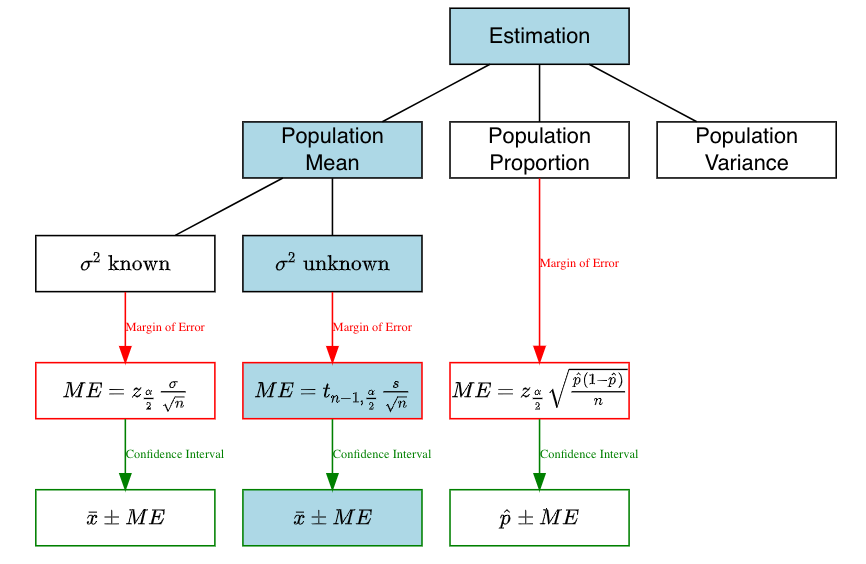
\includegraphics[width=0.9\linewidth]{pictures/EstimationGuide-Case2} \end{center}
\end{frame}

\hypertarget{exercise-2.-confidence-intervals.}{%
\section{Exercise 2. Confidence
intervals.}\label{exercise-2.-confidence-intervals.}}

\begin{frame}{Part 1. Confidence intervals.}
\protect\hypertarget{part-1.-confidence-intervals.}{}
Behave ``as if'' we did not know that the population mean is 2 and
population variance is 1.

For each of the \(10\) samples, construct the \(90\%\) confidence
interval for the sample mean.
\end{frame}

\begin{frame}{Where we currently are}
\protect\hypertarget{where-we-currently-are-2}{}
\begin{center}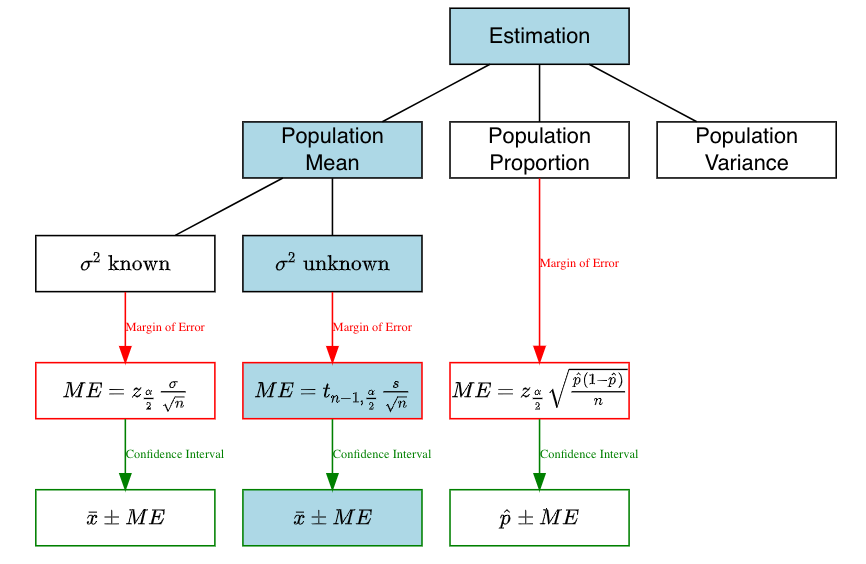
\includegraphics[width=0.9\linewidth]{pictures/EstimationGuide-Case2} \end{center}
\end{frame}

\begin{frame}{Part 2. Coverage.}
\protect\hypertarget{part-2.-coverage.}{}
\begin{itemize}
\item
  Now, we use again our knowledge about the true population mean. Using
  this information, fill in the blue row, indicating whether the
  confidence interval contains the true population mean (2).
\item
  Update the table a few times (for example, by refreshing the website)
  to see what happens. How often is the true population mean contained
  in the confidence interval?
\end{itemize}
\end{frame}

\hypertarget{exercise-3.-hypothesis-testing.}{%
\section{Exercise 3. Hypothesis
testing.}\label{exercise-3.-hypothesis-testing.}}

\begin{frame}{Exercise 3. Hypothesis testing.}
\begin{itemize}
\tightlist
\item
  Data set: \texttt{testscores.xls}

  \begin{itemize}
  \tightlist
  \item
    About: A sample (\(n=200\)) of student test scores in Math and
    English, drawn from a larger population.
  \item
    We know that the population standard deviation \(\sigma_\mu\) for
    variable ``English'' is equal to \(4.6\).
  \end{itemize}
\end{itemize}

\vspace{3mm}

\begin{itemize}
\tightlist
\item
  We want to test the following hypothesis at the \(5\%\) significance
  level:

  \begin{itemize}
  \tightlist
  \item
    \(H_0:\) The population mean for variable ``English'' is equal to
    \(73.5\).
  \item
    \(H_1:\) The population mean for variable ``English'' is different
    from \(73.5\). Run the test using either the ``critical values
    approach'' or the ``p-value approach'' depending on what you prefer.
  \end{itemize}
\end{itemize}
\end{frame}

\begin{frame}{Where we currently are}
\protect\hypertarget{where-we-currently-are-3}{}
\begin{center}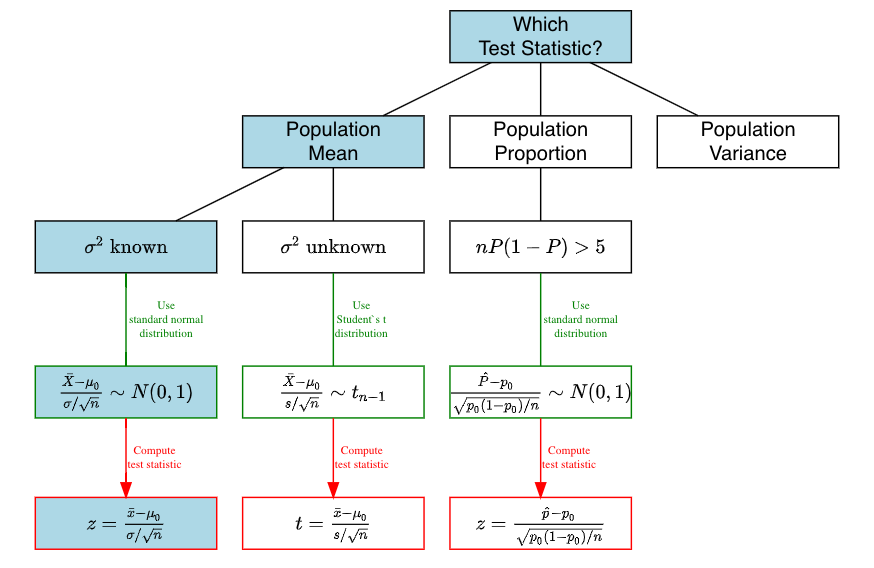
\includegraphics[width=0.9\linewidth]{pictures/HypothesisTestsGuide-Case1} \end{center}
\end{frame}

\begin{frame}{Tests of the Mean of a Normal Distribution Sigma Known}
\protect\hypertarget{tests-of-the-mean-of-a-normal-distribution-sigma-known}{}
Procedure includes 5 steps:

\begin{itemize}
\tightlist
\item
  Null hypothesis \(H_0\)
\item
  Alternative hypothesis \(H_1\)
\item
  Test statistic
\item
  Decision rule
\item
  Conclusion
\end{itemize}
\end{frame}

\begin{frame}{Tests of the Mean of a Normal Distribution Sigma Known}
\protect\hypertarget{tests-of-the-mean-of-a-normal-distribution-sigma-known-1}{}
Denote \(\mu\) the true population mean of English score.

\begin{itemize}
    \item [$\square$] Null hypothesis $H_0$:\\
      $H_0$: The population mean of "English" is equal to $73.5$.\\  
      $H_0$: $\mu = 73.5$
    \vspace{2mm}
    \item [$\square$] Alternative hypothesis $H_1$:\\
      $H_1$: The population mean of "English" is different from $73.5$.\\  
      $H_1$: $\mu \neq 73.5$
    \vspace{2mm}
    \item Test statistic
    \item Decision rule
    \item Conclusion
\end{itemize}
\end{frame}

\begin{frame}{Tests of the Mean of a Normal Distribution Sigma Known}
\protect\hypertarget{tests-of-the-mean-of-a-normal-distribution-sigma-known-2}{}
Denote \(\mu\) the true population mean of English score.

\begin{itemize}
    \item [$\square$] Null hypothesis $H_0$:\\
      $H_0$: The population mean of "English" is equal to $73.5$.\\  
      $H_0$: $\mu = 73.5$
    \vspace{2mm}
    \item [$\square$] Alternative hypothesis $H_1$:\\
      $H_1$: The population mean of "English" is different from $73.5$.\\  
      $H_1$: $\mu \neq 73.5$\\
      $\Rightarrow$ This is a two-tailed test.
    \vspace{2mm}
    \item Test statistic
    \item Decision rule
    \item Conclusion
\end{itemize}
\end{frame}

\begin{frame}{Test statistic}
\protect\hypertarget{test-statistic}{}
Given the sample size and the sampling scheme, the sample average is
asymptotically normally distributed: \[
Z =\frac{\bar{X}-\mu_0}{\sigma/\sqrt{n}} \sim N(0,1)
\]

We compute the z-score of the observation: \[
z = \frac{\bar{x}-\mu_0}{\sigma/\sqrt{n}} = \frac{73.74-73.5}{4.6/\sqrt{200}} \approx 0.738
\]
\end{frame}

\begin{frame}{Decision Rule}
\protect\hypertarget{decision-rule}{}
\begin{itemize}
    \item We are conducting a two-tailed test (\textit{look again $H_1$})\\
    \item The significance level $\alpha$ = 0.05\\
    \item Is the decision rule based on \textcolor{green}{\textbf{critical values}} or \textcolor{red}{\textbf{p-value}}?\\
\end{itemize}
\end{frame}

\begin{frame}[fragile]{Decision Rule - (1) Critical values approach}
\protect\hypertarget{decision-rule---1-critical-values-approach}{}
For two-tailed test, reject \(H_0\) if

\[
z = \frac{\bar{x}-\mu_0}{\sigma/\sqrt{n}} < -z_{\frac{\alpha}{2}} \text{ or } z = \frac{\bar{x}-\mu_0}{\sigma/\sqrt{n}} > z_{\frac{\alpha}{2}}
\]

\vspace{2mm}

\begin{itemize}
\tightlist
\item
  Compute critical value:\\
  \(z_{\frac{\alpha}{2}} = z_{\frac{0.05}{2}} = z_{0.025} = 1.96\)\\
  (\texttt{Excel} function: \(=\text{NORM.INV}(0.975,0,1)\)).
\end{itemize}

\vspace{2mm}

\begin{itemize}
\tightlist
\item
  Compare test statistic to critical value:\\
  Notice that \(z \approx 0.738\), which is greater than \(-1.96\)
  (\(-z_{0.025}\)) and less than \(1.96\) (\(z_{0.025}\))\\
  \(\Rightarrow\) We DO NOT reject \(H_0\) at \(\alpha = 0.05\).
\end{itemize}
\end{frame}

\begin{frame}[fragile]{Decision Rule - (2) P-value approach}
\protect\hypertarget{decision-rule---2-p-value-approach}{}
P-value corresponds to the probability of finding something more extreme
than the observed result, under the assumption that the null hypothesis
is true.

\vspace{2mm}

For two-tailed test, reject \(H_0\) if \(p-value \leq \alpha\).

\vspace{2mm}

\begin{itemize}
\item
  Compute p-value associated with the test statistics
  \(z \approx 0.738\): \[
  p-value = \text{Pr}(Z \leq -0.738) + \text{Pr}(Z \geq 0.738) \approx 2\times 0.23 = 0.46
  \] (\texttt{Excel} function:
  \(=\text{NORM.DIST}(-0.738,0,1,\text{TRUE})\))
\item
  Compare test statistic to the chosen \(\alpha\): The p-value
  (\(0.46\)) is larger than \(\alpha = 0.05\). \(\Rightarrow\) We DO NOT
  reject \(H_0\) at \(\alpha = 0.05\) (the same as Critical values
  approach).
\end{itemize}
\end{frame}

\begin{frame}{Decision Rule - Two Equivalent Approaches}
\protect\hypertarget{decision-rule---two-equivalent-approaches}{}
\begin{center}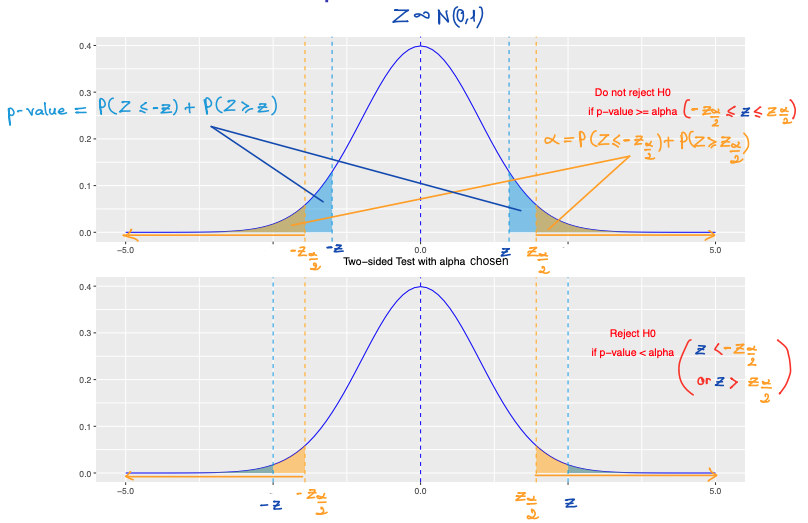
\includegraphics[width=0.9\linewidth]{pictures/Two-tailedTestRule} \end{center}
\end{frame}

\begin{frame}{Conclusion}
\protect\hypertarget{conclusion}{}
We maintain the null hypothesis. We do not reject the claim that the
population mean is equal to 73.5.
\end{frame}

\hypertarget{brief-review}{%
\section{BRIEF REVIEW}\label{brief-review}}

\begin{frame}{Estimation}
\protect\hypertarget{estimation}{}
\begin{center}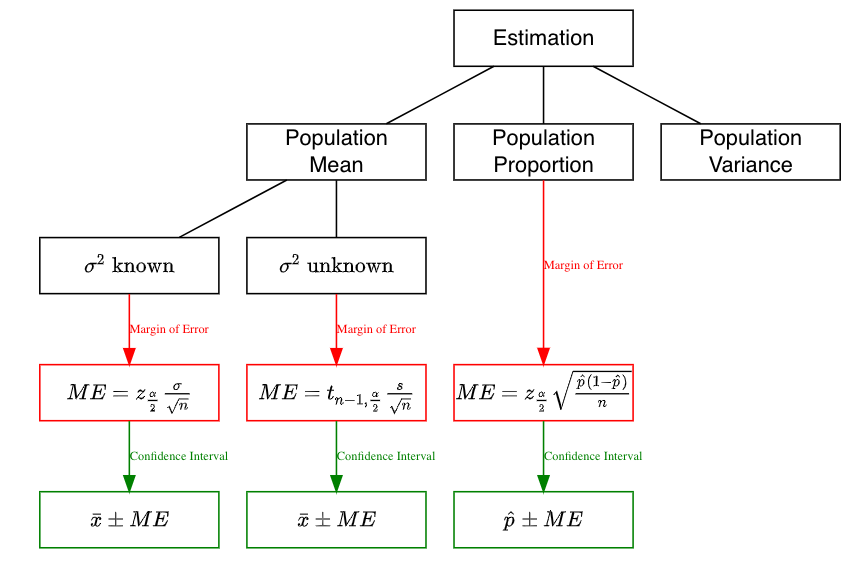
\includegraphics[width=0.9\linewidth]{pictures/EstimationGuide} \end{center}
\end{frame}

\begin{frame}{Hypothesis Testing}
\protect\hypertarget{hypothesis-testing}{}
\begin{center}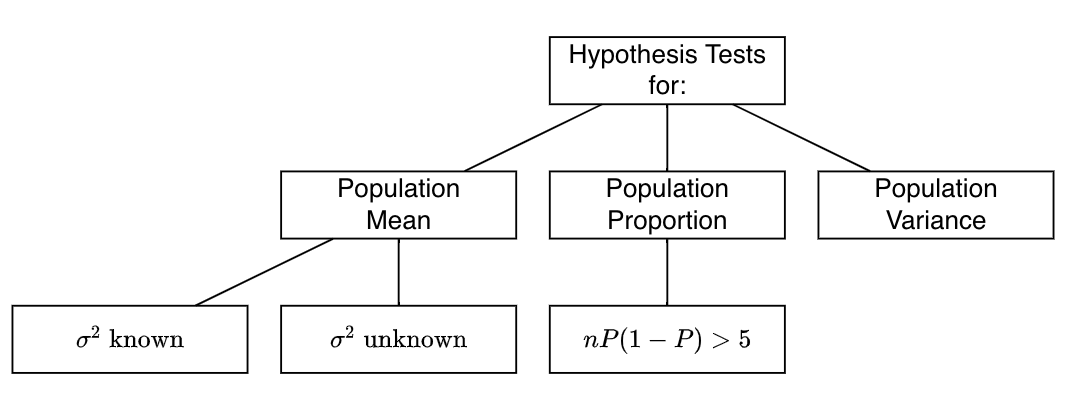
\includegraphics[width=0.9\linewidth]{pictures/HypothesisTestObj} \end{center}
\end{frame}

\begin{frame}{Hypothesis Testing}
\protect\hypertarget{hypothesis-testing-1}{}
General procedure includes 5 steps:

\begin{itemize}
\tightlist
\item
  Null hypothesis \(H_0\)
\item
  Alternative hypothesis \(H_1\)
\item
  Test statistic
\item
  Decision rule
\item
  Conclusion
\end{itemize}
\end{frame}

\begin{frame}{Hypothesis Testing}
\protect\hypertarget{hypothesis-testing-2}{}
\begin{center}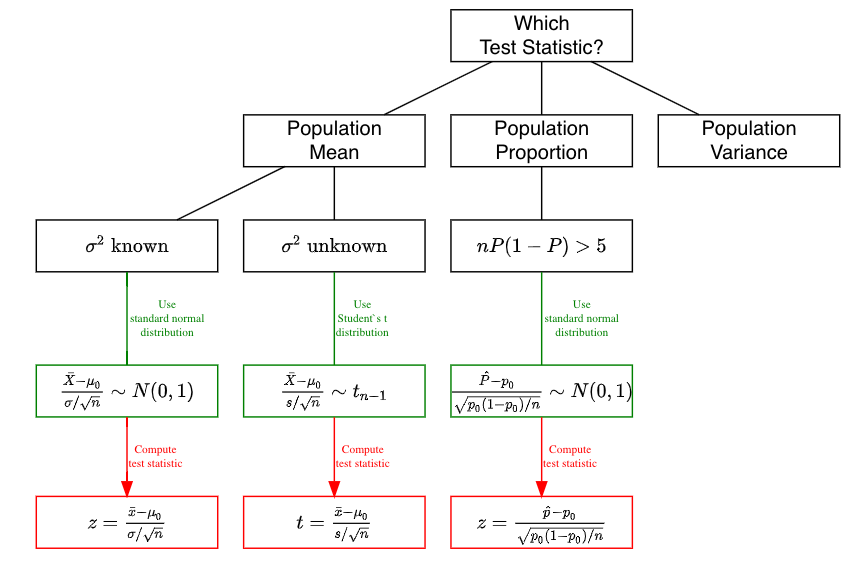
\includegraphics[width=0.9\linewidth]{pictures/HypothesisTestsGuide} \end{center}
\end{frame}

\begin{frame}{Tests of the Mean of a Normal Distribution Sigma Known}
\protect\hypertarget{tests-of-the-mean-of-a-normal-distribution-sigma-known-3}{}
Procedure includes 5 steps:

\begin{itemize}
\tightlist
\item
  Null hypothesis \(H_0\)
\item
  Alternative hypothesis \(H_1\)
\item
  Test statistic
\item
  Decision rule
\item
  Conclusion
\end{itemize}
\end{frame}

\begin{frame}{Tests of the Mean of a Normal Distribution Sigma Known}
\protect\hypertarget{tests-of-the-mean-of-a-normal-distribution-sigma-known-4}{}
Procedure includes 5 steps:

\begin{itemize}
    \item [$\square$] Null hypothesis $H_0$:\\
    $$
    H_0: \mu = \mu_{0}
    $$
    where $\mu_{0}$ is a hypothesized value.
    \item Alternative hypothesis $H_1$
    \item Test statistic
    \item Decision rule
    \item Conclusion
\end{itemize}
\end{frame}

\begin{frame}{Tests of the Mean of a Normal Distribution Sigma Known}
\protect\hypertarget{tests-of-the-mean-of-a-normal-distribution-sigma-known-5}{}
Procedure includes 5 steps:

\begin{itemize}
    \item [$\square$] Null hypothesis $H_0$:\\
    $$
    H_0: \mu = \mu_{0}
    $$
    where $\mu_{0}$ is a hypothesized value.
    \item [$\square$] Alternative hypothesis $H_1$:
    \vspace{2mm}
    \begin{center}
    \begin{tabular}{|c|c|}
    \hline
    Test & $H_1$\\
    \hline
    Two-sided &  $\mu \neq \mu_{0}$ \\
    \hline 
    Lower-tail & $\mu < \mu_{0}$\\
    \hline 
    Upper-tail & $\mu > \mu_{0}$\\ 
    \hline
    \end{tabular}
    \end{center}
    \vspace{2mm}
    \item Test statistic
    \item Decision rule
    \item Conclusion
\end{itemize}
\end{frame}

\begin{frame}{Tests of the Mean of a Normal Distribution Sigma Known}
\protect\hypertarget{tests-of-the-mean-of-a-normal-distribution-sigma-known-6}{}
Procedure includes 5 steps:

\begin{itemize}
    \item Null hypothesis $H_0$
    \item Alternative hypothesis $H_1$
    \item Test statistic
    \item [$\square$] Decision rule:
    \begin{itemize}
        \item Is this a two-sided test or an one-sided (lower-tail/upper-tail) test?\\
        $\Longrightarrow$ Look again $H_1$.
        \item What is the \textbf{significance level} $\alpha$?\\
        $\Longrightarrow$ Usually chosen to be 0.01, 0.05 or 0.10.
        \item Is the decision rule based on \textcolor{green}{\textbf{critical values}} or \textcolor{red}{\textbf{p-value}}?\\
        $\Longrightarrow$ Distinguish...
    \end{itemize}
    \item Conclusion
\end{itemize}
\end{frame}

\begin{frame}{Decision Rule - Two Equivalent Approaches}
\protect\hypertarget{decision-rule---two-equivalent-approaches-1}{}
\begin{center}
Approach 1: \textcolor{green}{\textbf{Critical-value Test}}\\
\vspace{3mm}
\begin{tabular}{|c|c|c|}
\hline
Test & $H_1$ & Reject $H_0$ if\\
\hline
Two-sided &  $\mu \neq \mu_{0}$ & $z^s < -z_{\frac{\alpha}{2}}$ or $ z^s> z_{\frac{\alpha}{2}}$\\
\hline 
Lower-tail & $\mu < \mu_{0}$ & $z^s < - z_{\alpha}$\\ 
\hline 
Upper-tail & $\mu > \mu_{0}$ & $z^s > z_{\alpha}$\\ 
\hline
\end{tabular}
\end{center}

\vspace{3mm}

\begin{center}
Approach 2: \textcolor{red}{\textbf{p-value Test}}\\
\vspace{3mm}
\begin{tabular}{|c|c|c|c|}
\hline
Test & $H_1$ & p-value & Reject $H_0$ if\\
\hline
Two-sided &  $\mu \neq \mu_{0}$ & \makecell{sum probabilities to the right \\ of $|z^s|$ and to the left of $-|z^s|$} & p-value $\leq \alpha$\\
    \hline 
Lower-tail & $\mu < \mu_{0}$ & probability to the left of $z^s$ & p-value $\leq \alpha$\\ 
\hline 
Upper-tail & $\mu > \mu_{0}$ & probability to the right of $z^s$ & p-value $\leq \alpha$\\ 
\hline
\end{tabular}
    
\vspace{1mm}
 
 \footnotesize   
*Note: p-value is probability of obtaining a test statistic more extreme ($\leq$ or $\geq$) than the observed sample value given $H_0$ is true.
\end{center}
\end{frame}

\begin{frame}{Tests of the Mean of a Normal Distribution Sigma Known}
\protect\hypertarget{tests-of-the-mean-of-a-normal-distribution-sigma-known-7}{}
Procedure includes 5 steps:

\begin{itemize}
    \item Null hypothesis $H_0$
    \item Alternative hypothesis $H_1$
    \item Test statistic
    \item Decision rule
    \item [$\square$] Conclusion:
    \begin{itemize}
        \item Do you \textit{reject} or or \textit{fail to reject} the null hypothesis at the significance level $\alpha$?
    \end{itemize}
\end{itemize}
\end{frame}

\hypertarget{excel-notes}{%
\section{EXCEL NOTES}\label{excel-notes}}

\begin{frame}[fragile]{Relevant functions (I)}
\protect\hypertarget{relevant-functions-i}{}
\normalsize

Launch the \textbf{Excel} online

\footnotesize

\textcolor{blue}{https://www.office.com/launch/excel?auth=2}

\vspace{3mm}

\normalsize

\textcolor{red}{NORM.INV()} \footnotesize To return the inverse of the
normal cumulative distribution for the specified mean and standard
deviation (\emph{real number}).

\begin{Shaded}
\begin{Highlighting}[]
\NormalTok{= NORM.INV(probability,mean,standard\_dev)}
\end{Highlighting}
\end{Shaded}

\normalsize

\textcolor{red}{T.INV()} \footnotesize To return the t-value of the
Student's t-distribution as a function of the probability and the
degrees of freedom (\emph{real number}).

\begin{Shaded}
\begin{Highlighting}[]
\NormalTok{= T.INV(probability,degrees\_freedom)}
\end{Highlighting}
\end{Shaded}

\normalsize

\textcolor{red}{NORMSDIST()} \footnotesize To return the standard normal
cumulative distribution (\emph{probability}).

\begin{Shaded}
\begin{Highlighting}[]
\NormalTok{= NORMSDIST(z)}
\end{Highlighting}
\end{Shaded}
\end{frame}

\begin{frame}[fragile]{Relevant functions (II)}
\protect\hypertarget{relevant-functions-ii}{}
\normalsize

Launch the \textbf{Excel} online

\footnotesize

\textcolor{blue}{https://www.office.com/launch/excel?auth=2}

\vspace{3mm}

\normalsize

\textcolor{red}{NORM.INV(RAND())} \footnotesize To draws a random
variable from the normal distribution with the specified mean and
standard deviation (\emph{real number}).

\begin{Shaded}
\begin{Highlighting}[]
\NormalTok{= NORM.INV(RAND(),mean,standard\_dev)}
\end{Highlighting}
\end{Shaded}
\end{frame}

\end{document}
